\chapter{Preliminary work:}
We have already conducted an eye-tracking experiment and collected DOI data from it~\cite{Ala16}. We demonstrated that the collected DOI data supports our claims for Contribution-1. In the experiment, we instrumented a PivotPaths visualization which is generated from popular IMDB data. Additionally, we implemented all of the three viewed-object-detection algorithms which are discussed in Section 3.1. Afterward, we conducted the experiment on 9 adult users. The users were asked to perform visual tasks related to movies using the instrumented visualization. We collected DOI data in addition with gaze samples, and screen-video of the experimental sessions. Each user participated for approximately one hour session. Next, we investigated the reliability of the collected DOI data in two alternate ways. First, we validated our methodologies of DOI data collection by comparing with manual human annotation. Second, we investigated whether the collected data is relevant with the given task descriptions. The results were published in IEEE TVCG. 

\section{Validation of DOI Methodologies using Human Annotation}
We asked five human annotators to analyze the collected video recordings overlaid with gaze samples to annotate which objects are viewed. For time constraints, we asked each human annotator to annotate a three-minute video of a task session, for six random users. Human annotators were provided a special interface so that they can play the video backward and forward with minimum 100ms time-step. Annotators spent approximately one hour for each video. Four annotators completed all videos from six users while one annotator was able to annotate three of them. 

Afterward, the annotation data of each user was transformed in temporal vectors with 100ms resolutions. Then, we created a similar representation for the automatically collected DOI data for each DOI collection method (i.e. AOI, Probabilistic, and Intelligent).  For each collection method, we computed the similarity between its output and human annotation data. Then, we calculated the average similarity for each method. Next, we calculated similarity among the different human annotations. Then, we calculated an average similarity score among human annotations. We plot all these similarity scores in Figure~\ref{fig:Similarity}. 

\begin{figure}[htb]
  \centering
  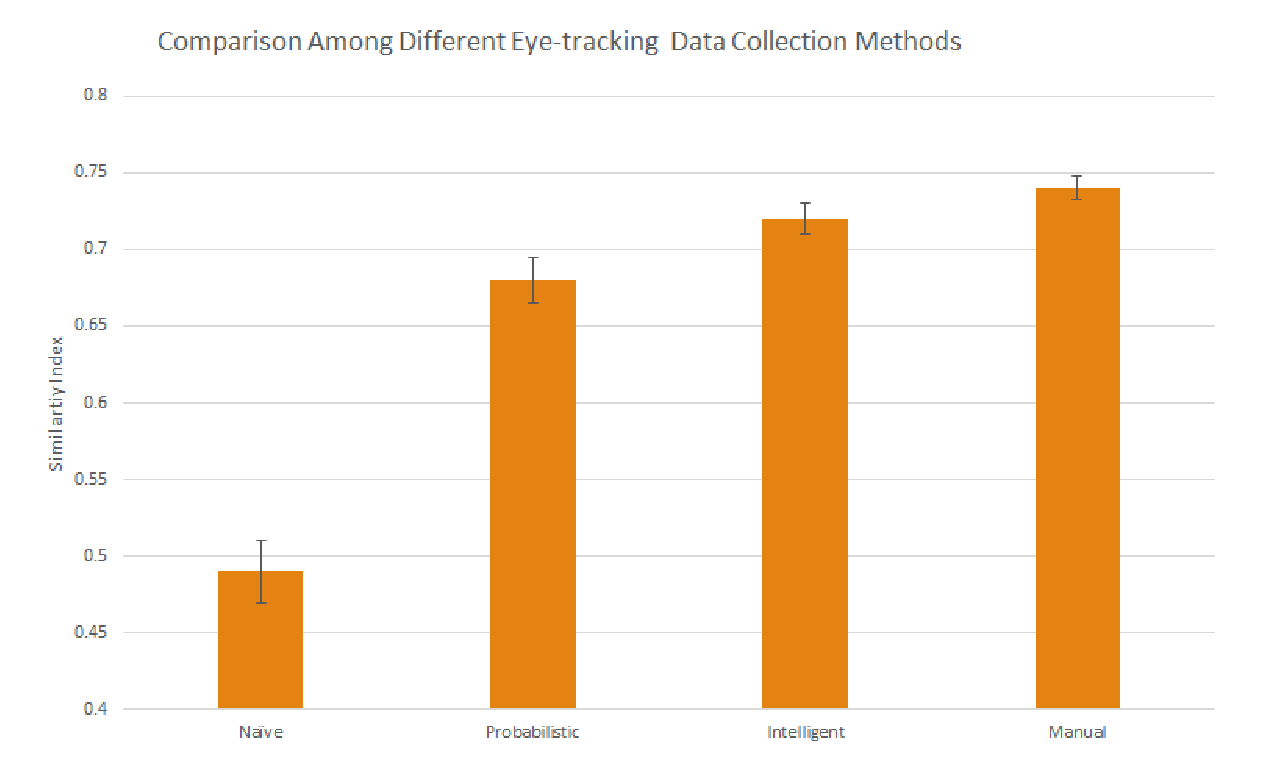
\includegraphics[width=0.99\linewidth]{images/Similarity.eps}
  \caption{: Similarity scores plotted for three different algorithms and Human annotators.}
	\label{fig:Similarity}
\end{figure}

In Figure~\ref{fig:Similarity}, we can observe that human annotators are more similar among themselves than Intelligent, Probabilistic approaches. AOI approach is the least similar to the human annotation data. In conclusion, we demonstrated that collected DOI data with the intelligent approach is likely to be the most reliable method of DOI data collection. 

\section{DOI Data is Relevant to Given Task Description}
In the experiment, users were asked to perform four different visual tasks regarding certain movie elements (i.e. titles, actors, directors, and genres). One of the tasks we used in the experiment involved the movies: `Indiana Jones and the Last Crusade', `Raiders of the Lost Ark', and `Star Wars Episode V'. Figure~\ref{fig:heatmap} is a heatmap generated from DOI data of a user performing that task. The heatmap depicts which movie elements are mostly viewed by the user over time. In Figure~\ref{fig:heatmap}, we can see that all of the above-mentioned movies are mostly viewed. Thus, we infer that the data collected for this particular task for this user is relevant. 


\begin{figure}[htb]
  \centering
  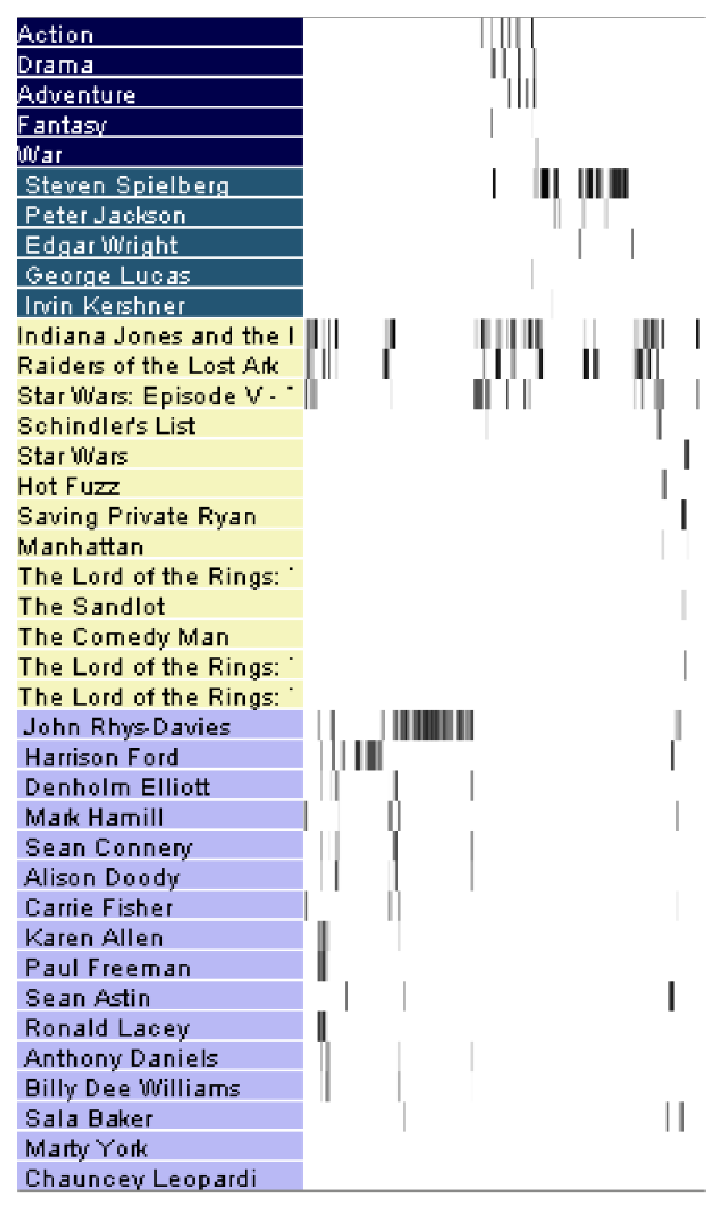
\includegraphics[width=0.6\linewidth]{images/heatmap.eps}
  \caption{: Heatmap showing movie elements viewed over time. We can see Indiana Jones, Raiders of the Lost Ark, Star Wars Episode V is viewed mostly over time. }
	\label{fig:heatmap}
\end{figure}

\begin{figure}[htb]
  \centering
  \includegraphics[width=0.6\linewidth]{images/Relevance.eps}
  \caption{: User interest vs relevance score for four types of tasks. }
	\label{fig:Relevance}
\end{figure}

In Figure~\ref{fig:Relevance}, we plot users' interests against relevance scores for four types of tasks. We can observe, all of the plots depicts the same pattern where users looked at relevant objects with more interests. Thus, we conclude that our collected DOI data is relevant, and was collected in a reliable way.  
